\chapter{Ход работы}

\section{Задание 0}

Ниже приведен дизассмблированный код общей программы, получен\-ный 
в результате выполнения команды make.

\begin{lstlisting}[label={common_asm}, language={RISC-V}, caption=Дизассемблированный код общей программы]
SYMBOL TABLE:
80000000 l    d  .text  00000000 .text
80000040 l    d  .data  00000000 .data
00000000 l    df *ABS*  00000000 test.o
00000008 l       *ABS*  00000000 len
00000004 l       *ABS*  00000000 enroll
00000004 l       *ABS*  00000000 elem_sz
80000040 l       .data  00000000 _x
8000000c l       .text  00000000 loop
8000003c l       .text  00000000 forever
80000000 g       .text  00000000 _start
80000060 g       .data  00000000 _end

Disassembly of section .text:

80000000 <_start>:
80000000:       00200a13                addi    x20,x0,2
80000004:       00000097                auipc   x1,0x0
80000008:       03c08093                addi    x1,x1,60 # 80000040 <_x>

8000000c <loop>:
8000000c:       0000a103                lw      x2,0(x1)
80000010:       002f8fb3                add     x31,x31,x2
80000014:       0040a103                lw      x2,4(x1)
80000018:       002f8fb3                add     x31,x31,x2
8000001c:       0080a103                lw      x2,8(x1)
80000020:       002f8fb3                add     x31,x31,x2
80000024:       00c0a103                lw      x2,12(x1)
80000028:       002f8fb3                add     x31,x31,x2
8000002c:       01008093                addi    x1,x1,16
80000030:       fffa0a13                addi    x20,x20,-1
80000034:       fc0a1ce3                bne     x20,x0,8000000c <loop>
80000038:       001f8f93                addi    x31,x31,1

8000003c <forever>:
8000003c:       0000006f                jal     x0,8000003c <forever>

Disassembly of section .data:

80000040 <_x>:
80000040:       0001                    c.addi  x0,0
80000042:       0000                    c.unimp
80000044:       0002                    c.slli64        x0
80000046:       0000                    c.unimp
80000048:       00000003                lb      x0,0(x0) # 0 <elem_sz-0x4>
8000004c:       0004                    .2byte  0x4
8000004e:       0000                    c.unimp
80000050:       0005                    c.addi  x0,1
80000052:       0000                    c.unimp
80000054:       0006                    c.slli  x0,0x1
80000056:       0000                    c.unimp
80000058:       00000007                .4byte  0x7
8000005c:       0008                    .2byte  0x8
\end{lstlisting}

\clearpage
\section{Задание 1}

\begin{lstlisting}[label={common_asm}, language={RISC-V}, caption=Исходный текст программы для варианта 21]
    .section .text
    .globl _start;
    len = 8 # Размер массива
    enroll = 4 # Количество обрабатываемых элементов за одну итерацию
    elem_sz = 4 # Размер одного элемента массива

_start:
    la x1, _x
    addi x20, x0, (len-1)/enroll
    lw x31, 0(x1)
    addi x1, x1, elem_sz*1
lp:
    lw x2, 0(x1)
    lw x3, 4(x1)
    lw x4, 8(x1)
    lw x5, 12(x1)
    bltu x2, x31, lt1
    add x31, x0, x2
lt1:    bltu x3, x31, lt2
    add x31, x0, x3
lt2:    bltu x4, x31, lt3
    add x31, x0, x4 #!
lt3:    bltu x5, x31, lt4
    add x31, x0, x5
lt4:
    add x1, x1, elem_sz*enroll
    addi x20, x20, -1
    bne x20, x0, lp
lp2: j lp2

    .section .data
_x: .4byte 0x1
    .4byte 0x2
    .4byte 0x3
    .4byte 0x4
    .4byte 0x5
    .4byte 0x6
    .4byte 0x7
    .4byte 0x8
    .4byte 0x9

\end{lstlisting}

\clearpage

\begin{lstlisting}[label={common_disasm}, language={RISC-V}, caption=Дизассеблированный код программы для варианта 21]
SYMBOL TABLE:
80000000 l    d  .text  00000000 .text
80000054 l    d  .data  00000000 .data
00000000 l    df *ABS*  00000000 individual.o
00000008 l       *ABS*  00000000 len
00000004 l       *ABS*  00000000 enroll
00000004 l       *ABS*  00000000 elem_sz
80000054 l       .data  00000000 _x
80000014 l       .text  00000000 lp
8000002c l       .text  00000000 lt1
80000034 l       .text  00000000 lt2
8000003c l       .text  00000000 lt3
80000044 l       .text  00000000 lt4
80000050 l       .text  00000000 lp2
80000000 g       .text  00000000 _start
80000078 g       .data  00000000 _end

Disassembly of section .text:

80000000 <_start>:
80000000:       00000097                auipc   x1,0x0
80000004:       05408093                addi    x1,x1,84 # 80000054 <_x>
80000008:       00100a13                addi    x20,x0,1
8000000c:       0000af83                lw      x31,0(x1)
80000010:       00408093                addi    x1,x1,4

80000014 <lp>:
80000014:       0000a103                lw      x2,0(x1)
80000018:       0040a183                lw      x3,4(x1)
8000001c:       0080a203                lw      x4,8(x1)
80000020:       00c0a283                lw      x5,12(x1)
80000024:       01f16463                bltu    x2,x31,8000002c <lt1>
80000028:       00200fb3                add     x31,x0,x2

8000002c <lt1>:
8000002c:       01f1e463                bltu    x3,x31,80000034 <lt2>
80000030:       00300fb3                add     x31,x0,x3

80000034 <lt2>:
80000034:       01f26463                bltu    x4,x31,8000003c <lt3>
80000038:       00400fb3                add     x31,x0,x4

8000003c <lt3>:
8000003c:       01f2e463                bltu    x5,x31,80000044 <lt4>
80000040:       00500fb3                add     x31,x0,x5

80000044 <lt4>:
80000044:       01008093                addi    x1,x1,16
80000048:       fffa0a13                addi    x20,x20,-1
8000004c:       fc0a14e3                bne     x20,x0,80000014 <lp>

80000050 <lp2>:
80000050:       0000006f                jal     x0,80000050 <lp2>

Disassembly of section .data:

80000054 <_x>:
80000054:       0001                    c.addi  x0,0
80000056:       0000                    c.unimp
80000058:       0002                    c.slli64        x0
8000005a:       0000                    c.unimp
8000005c:       00000003                lb      x0,0(x0) # 0 <elem_sz-0x4>
80000060:       0004                    .2byte  0x4
80000062:       0000                    c.unimp
80000064:       0005                    c.addi  x0,1
80000066:       0000                    c.unimp
80000068:       0006                    c.slli  x0,0x1
8000006a:       0000                    c.unimp
8000006c:       00000007                .4byte  0x7
80000070:       0008                    .2byte  0x8
80000072:       0000                    c.unimp
80000074:       0009                    c.addi  x0,2
\end{lstlisting}

\clearpage

\begin{lstlisting}[label={common_c}, language={C}, caption=Псевдокод на языке C эквивалентной программы]
#define len 8
#define enroll 4
#define elem_sz 4
int _x[]={1,2,3,4,5,6,7,8};
void _start() {
    int x20 = len/enroll;
    int *x1 = _x;

    do {
        int x2 = x1[0];
        x31 += x2;
        x2 = x1[1];
        x31 += x2;
        x2 = x1[2];
        x31 += x2;
        x2 = x1[3];
        x31 += x2;
        x1 += enroll;
        x20--;
    } while(x20 != 0);
    x31++;
    while(1){}
}
\end{lstlisting}

\clearpage

\section{Задание 2}

Для выполнения задания 2 необходимо получить снимок экрана, 
содер\-жащий временную диаграмму выполнения стадий выборки и 
диспетчериза\-ции команды с указанным адресом.

Вариант 21:

\hspace{1cm} Адрес команды: 80000030, 2-я итерация

\hspace{1cm} Код команды: fffa0a13

\hspace{1cm} Команда: addi x20, x20, -1

\begin{figure}[ph!]
    \center{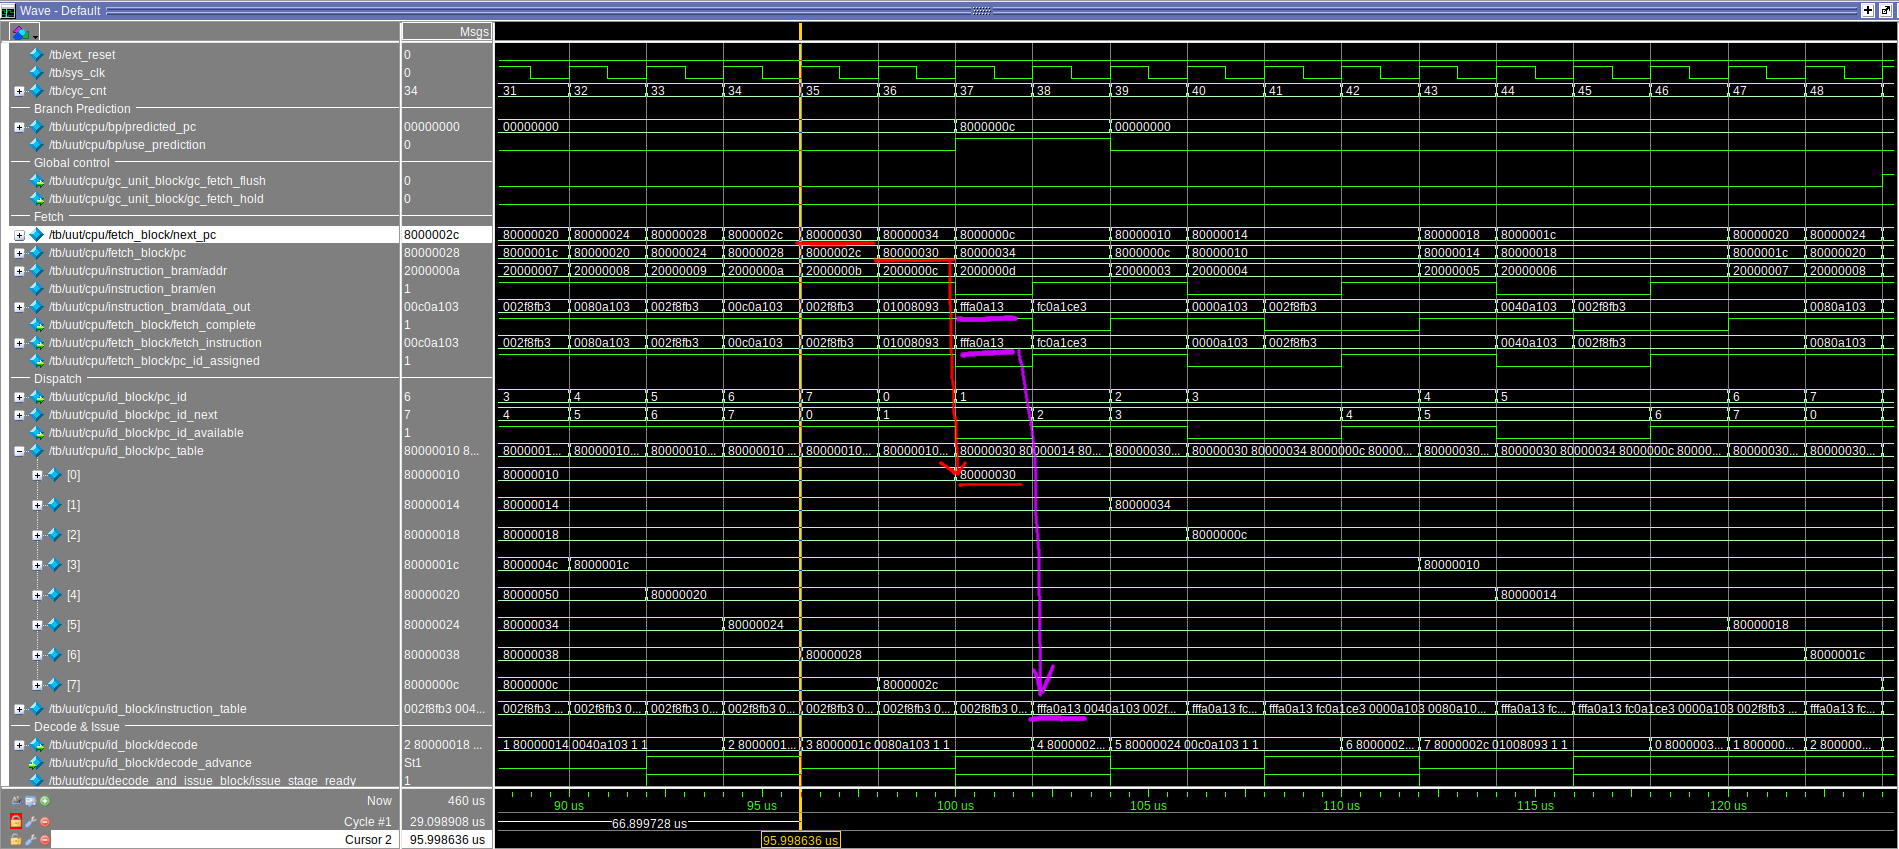
\includegraphics[scale=0.3]{images/задание2.png}}
    \caption{Временная диаграмма выборки и диспетчеризации команды}
\end{figure}

\clearpage

\section{Задание 3}
Для выполнения задания 3 необходимо получить снимок экрана,
содер\-жащий временную диаграмму выполнения стадии декодирования
и плани\-рования на выполнение команды с указанным адресом.

Вариант 21:

\hspace{1cm} Адрес команды, номер итерации: 80000018, 1-я.
 
\hspace{1cm} Код команды: 002f8fb3.
 
\hspace{1cm} Команда: add x31,x31,x2.

\begin{figure}[ph!]
    \center{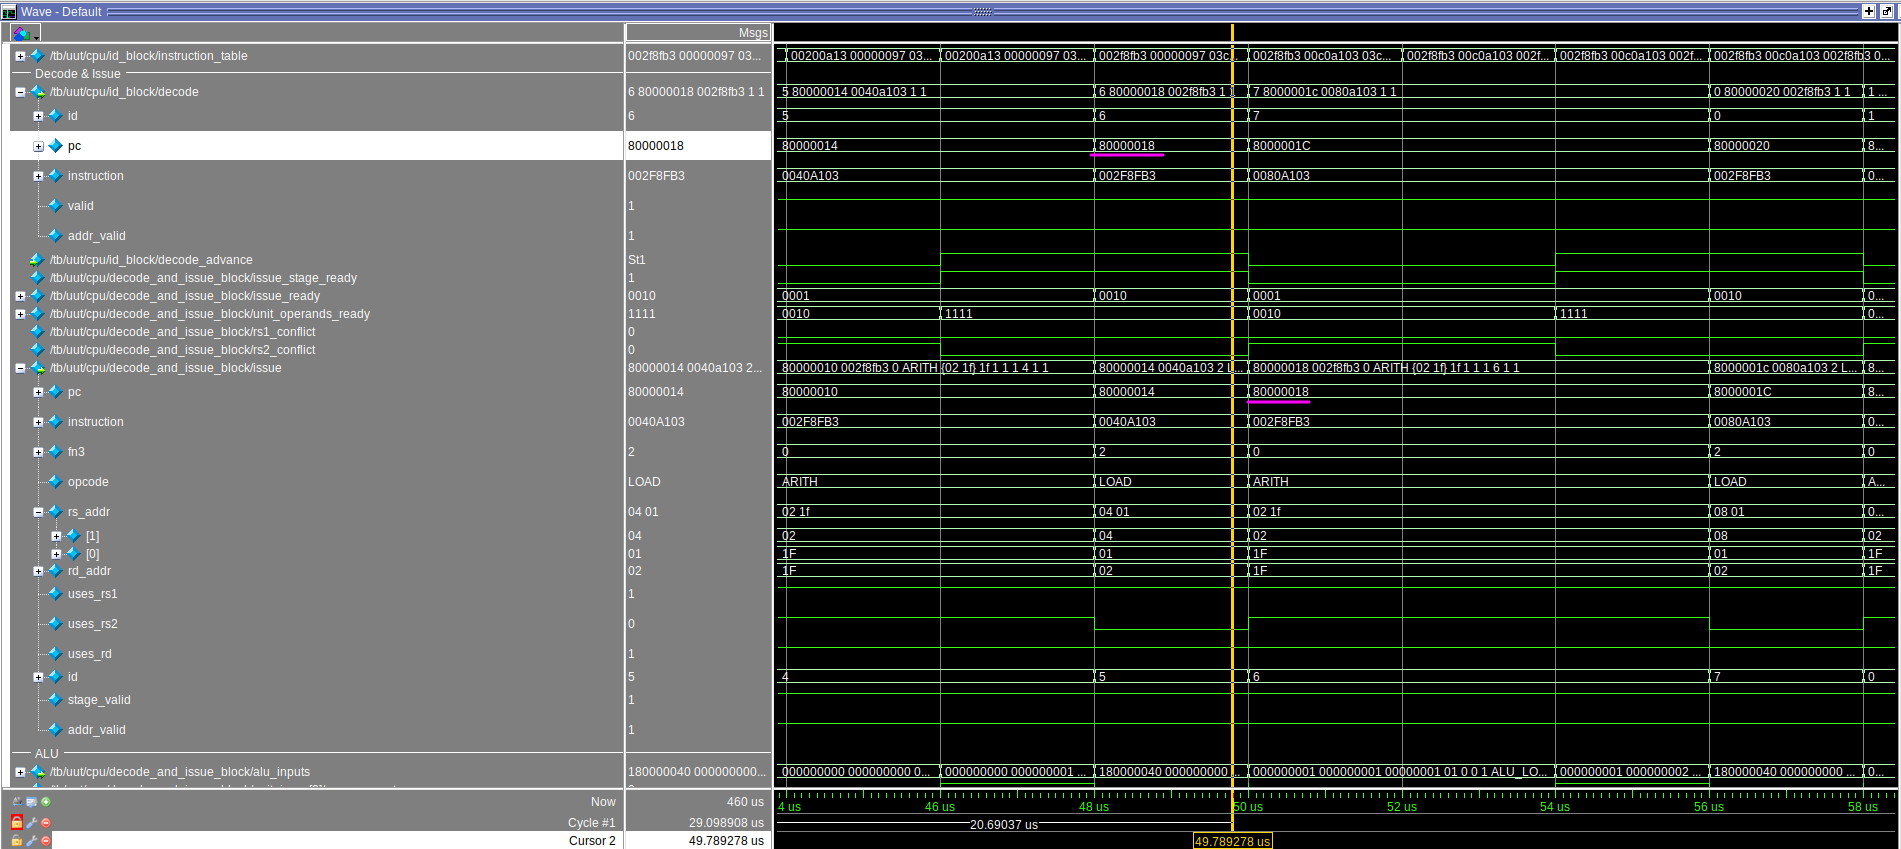
\includegraphics[scale=0.3]{images/задание3.png}}
    \caption{Временная диаграмма выполнения стадии декодирования и планирования на выполнение команды}
    \label{fig:task3}
\end{figure}

На этапе декодирования никаких конфликтов не возникает. 
На следую\-щем такте, когда происходит планирование на 
выполнение команды, сигнал rs2\_conflict выставляется в
единицу и сохраняет это значение еще один такт. 

Причина этому в том, что предыдущая команда lw x2,4(x1)
еще не закончила свое выполнение, а значит целевой для
обеих команд регистр x2 не может быть предоставлен еще
2 такта, поэтому и возникает конфликт.

\clearpage
\section{Задание 4}
Для выполнения задания 4 необходимо получить снимок экрана, содер\-жащий
временную диаграмму стадии выполнения команды с указанным
ад\-ресом.

Вариант 21:

\hspace{1cm} Адрес команды, номер итерации: 80000028, 2-я.
 
\hspace{1cm} Код команды: 002f8fb3.
 
\hspace{1cm} Команда: add x31,x31,x2.

\begin{figure}[ph!]
    \center{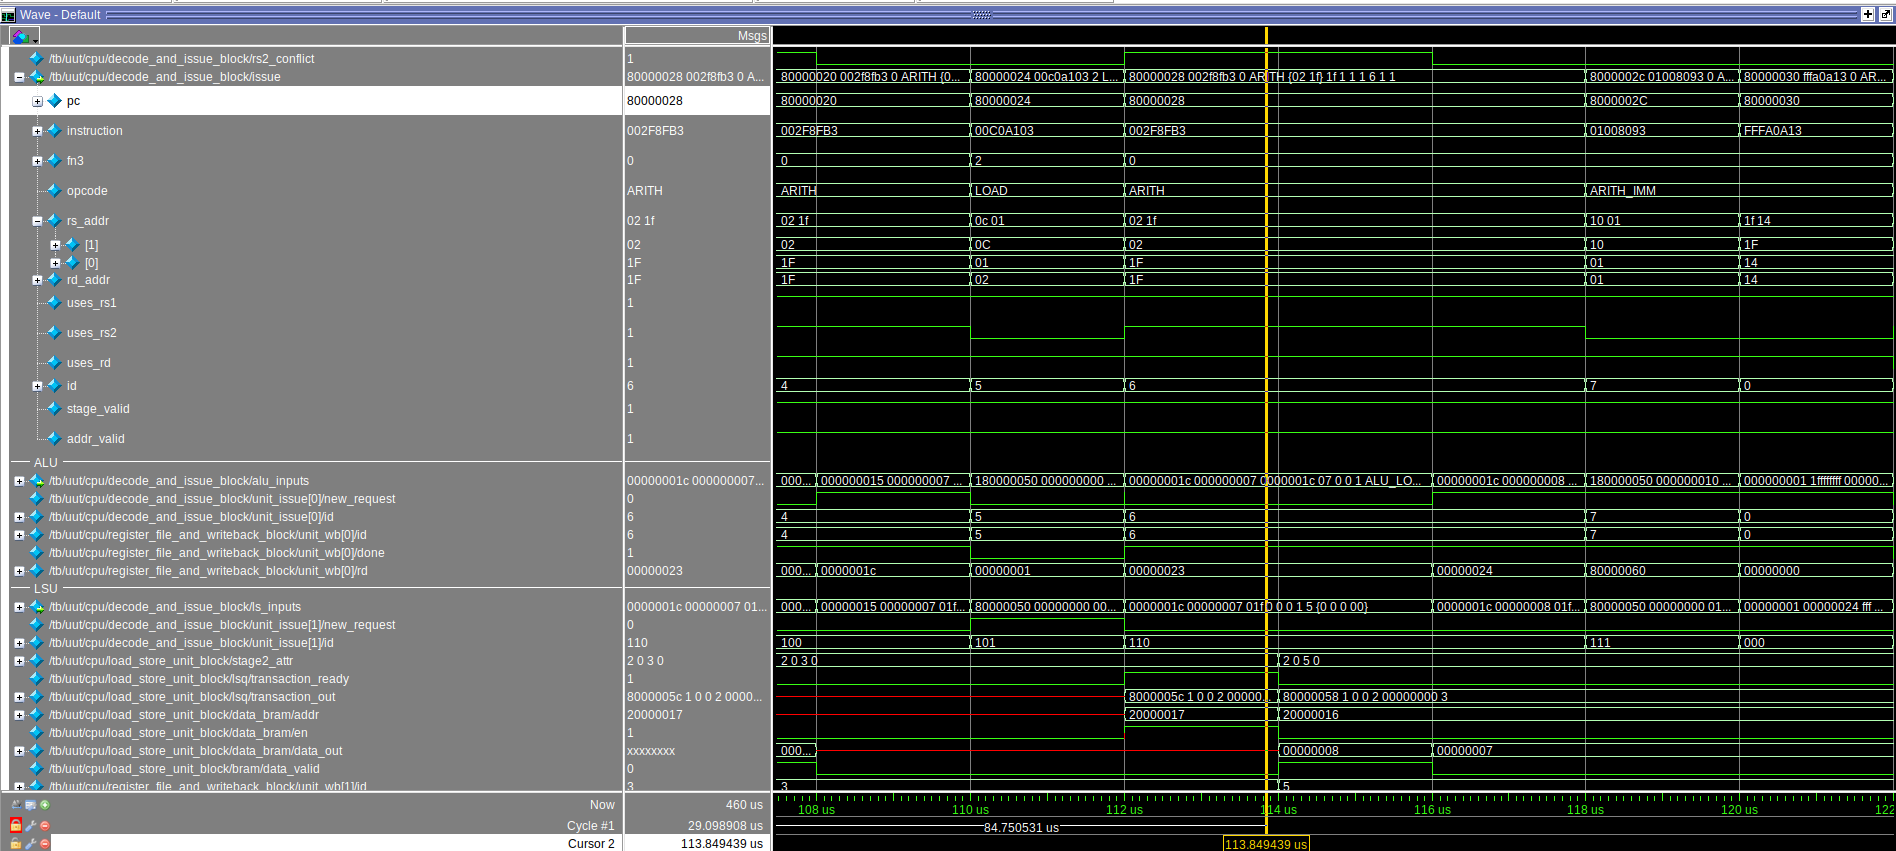
\includegraphics[scale=0.3]{images/задание4.png}}
    \caption{Выполнение команды с адресом 80000028}
\end{figure}

\clearpage
\section{Задание 5}

Данное задание связано с получением временных диаграмм для 
про\-граммы по варианту. Согласно полученным временным диаграммам
необхо\-димо построить трассу выполнения программы.

\subsection{Выполнение команды}

Ниже приведены временные диаграммы этапов выполнения команды
add x31,x0,x4 (адрес команды 80000038). 

\begin{figure}[ph!]
    \center{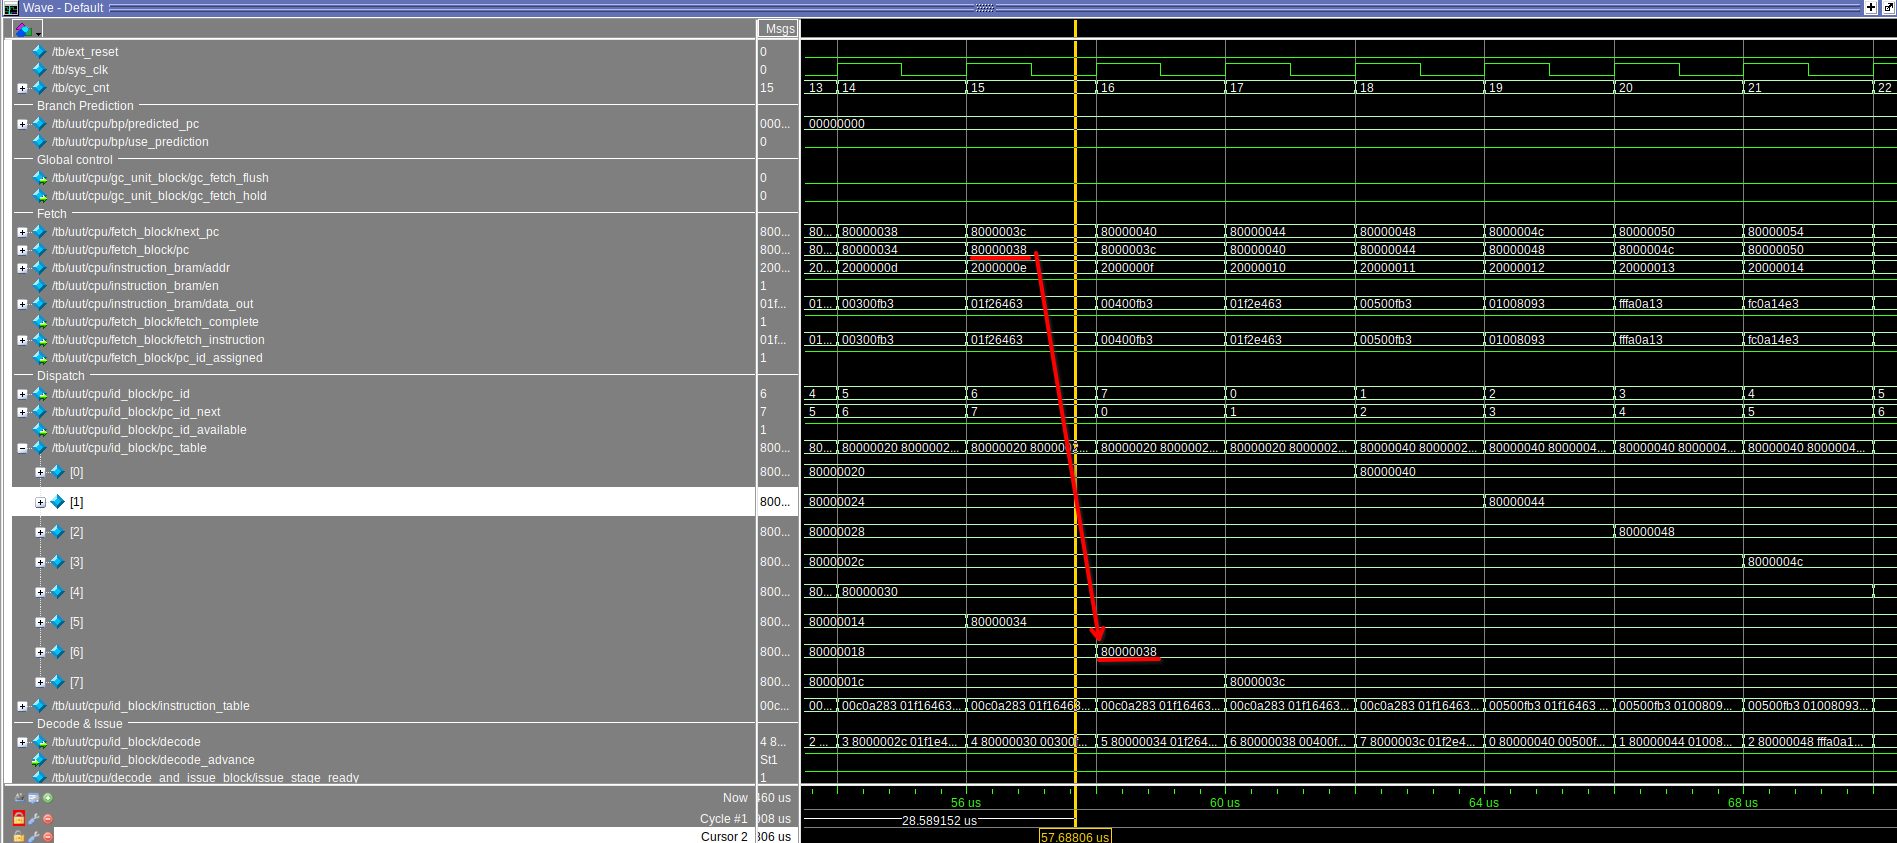
\includegraphics[scale=0.3]{images/задание5_1.png}}
    \caption{Выборка и диспетчеризация}
\end{figure}

\begin{figure}[ph!]
    \center{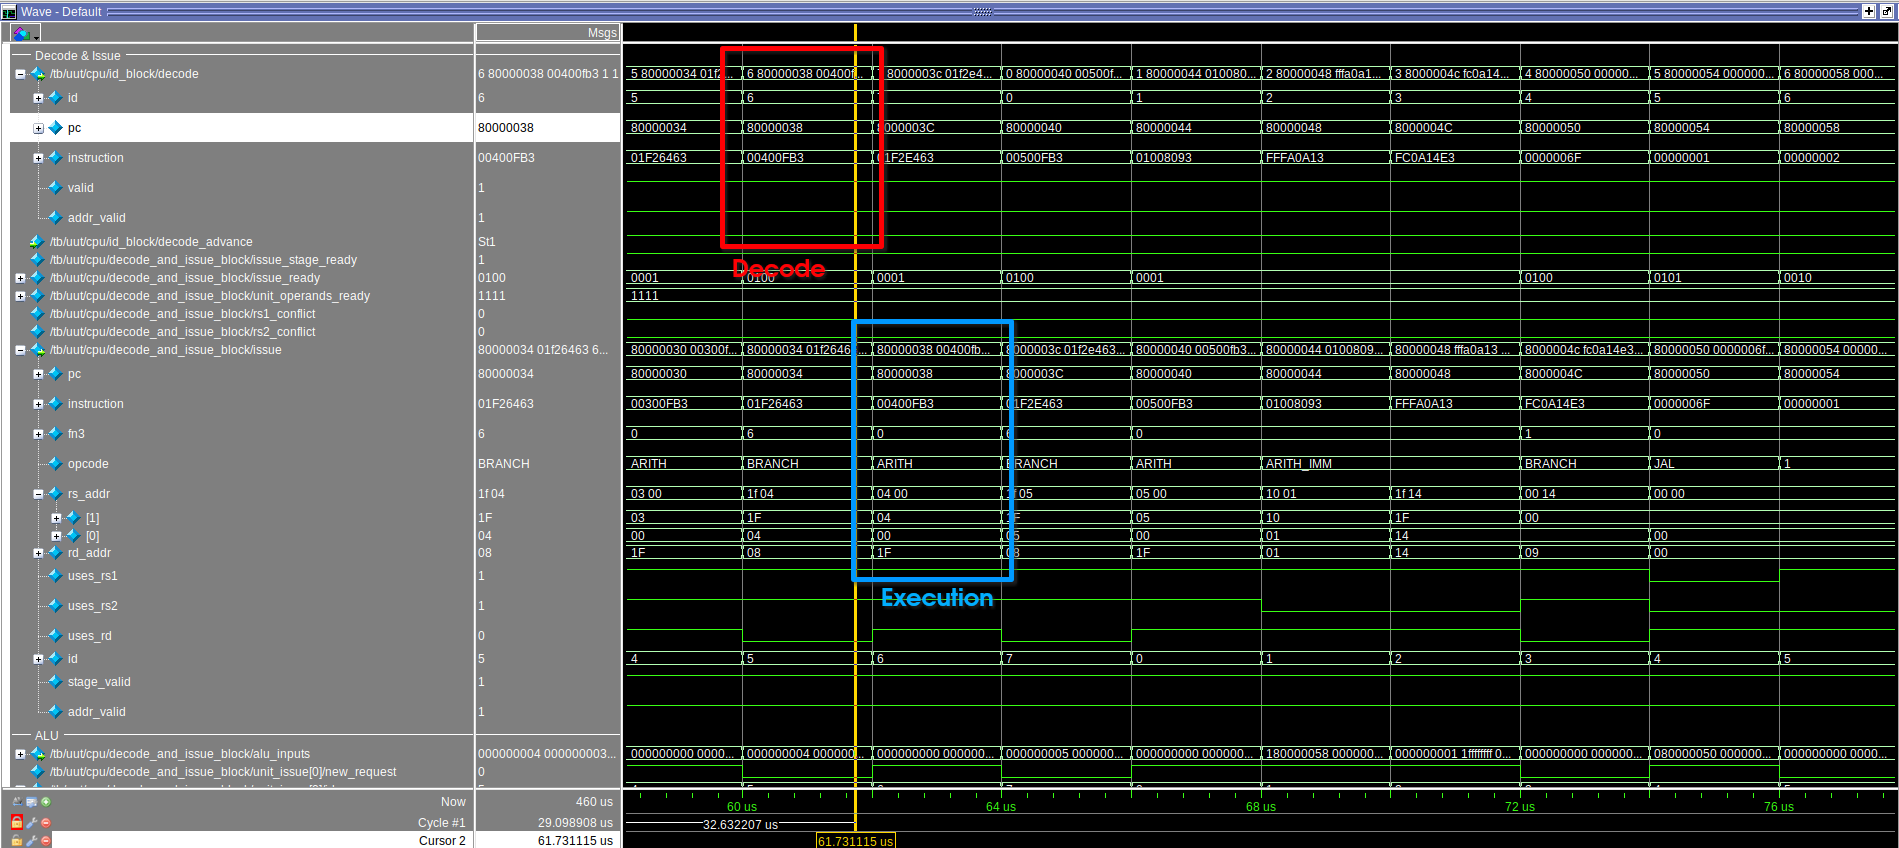
\includegraphics[scale=0.3]{images/задание5_2.png}}
    \caption{Декодирование и выполнение}
\end{figure}

\clearpage

\subsection{Регистр x31}

\begin{figure}[ph!]
    \center{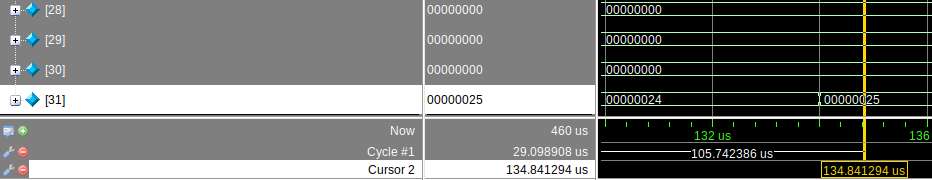
\includegraphics[scale=0.6]{images/x31_common.png}}
    \caption{Значение регистра x31 на момент завершения общей программы}
\end{figure}

\begin{figure}[ph!]
    \center{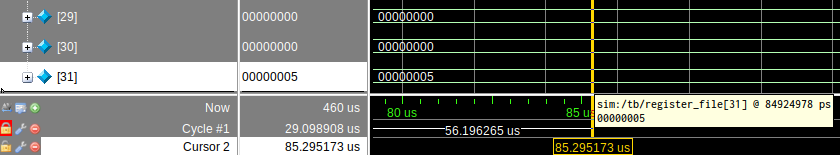
\includegraphics[scale=0.66]{images/x31_ind.png}}
    \caption{Значение регистра x31 на момент завершения программы по варианту}
\end{figure}


\clearpage
\subsection{Трасса выполнения программы}

\begin{figure}[h]
    \centering
    \includesvg[width=0.9\textwidth]{images/individual.svg}
    \caption{Трасса выполнения программы}
    \label{fig:trace}
\end{figure}

При составлении трассы, изображенной на рисунке \ref{fig:trace},
не было обнару\-жено ни одного конфликта, программа в оптимизации не
нуждается.
